\chapter*{Введение}

Уязвимость в веб приложении представляет собой слабое место или ошибку в его структуре, коде, конфигурации или бизнес логике, которая может быть использована злоумышленником для неправомерного доступа, модификации данных, отказа в обслуживании (DoS), или других видов атак. Уязвимости могут возникнуть из за неправильного проектирования, программирования, конфигурации или недостаточной защиты.

Исследование и устранение уязвимостей являются важной частью процесса обеспечения безопасности веб приложений. Разработчики, тестировщики безопасности и администраторы должны активно мониторить, анализировать и устранять потенциальные угрозы.

\chapter{Нарушенный контроль доступа}

относится к уязвимости в системе безопасности, которая возникает, когда механизмы контроля доступа системы не реализованы или не применены должным образом. Механизмы контроля доступа создаются для обеспечения того, чтобы только авторизованные пользователи или организации могли получать доступ к определенным ресурсам или выполнять определенные действия в системе. Когда контроль доступа нарушен, это означает, что злоумышленник может получить несанкционированный доступ к ресурсам или выполнить действия, которые он не должен иметь возможности.

Эта уязвимость может проявляться различными способами, такими как неадекватные механизмы аутентификации, отсутствие надлежащих проверок авторизации и ненадежный контроль доступа к конфиденциальным данным. Нарушение контроля доступа может иметь серьезные последствия, такие как утечка данных, кража конфиденциальной информации и несанкционированные изменения конфигурации системы. Это представляет собой серьезную угрозу безопасности, и ее следует устранить как можно скорее, чтобы предотвратить потенциальные атаки.

На рисунке (\ref{fig:mel-spec}) представлено, сделаны работы на OWASP: 
\begin{figure}[H]
	\centering
	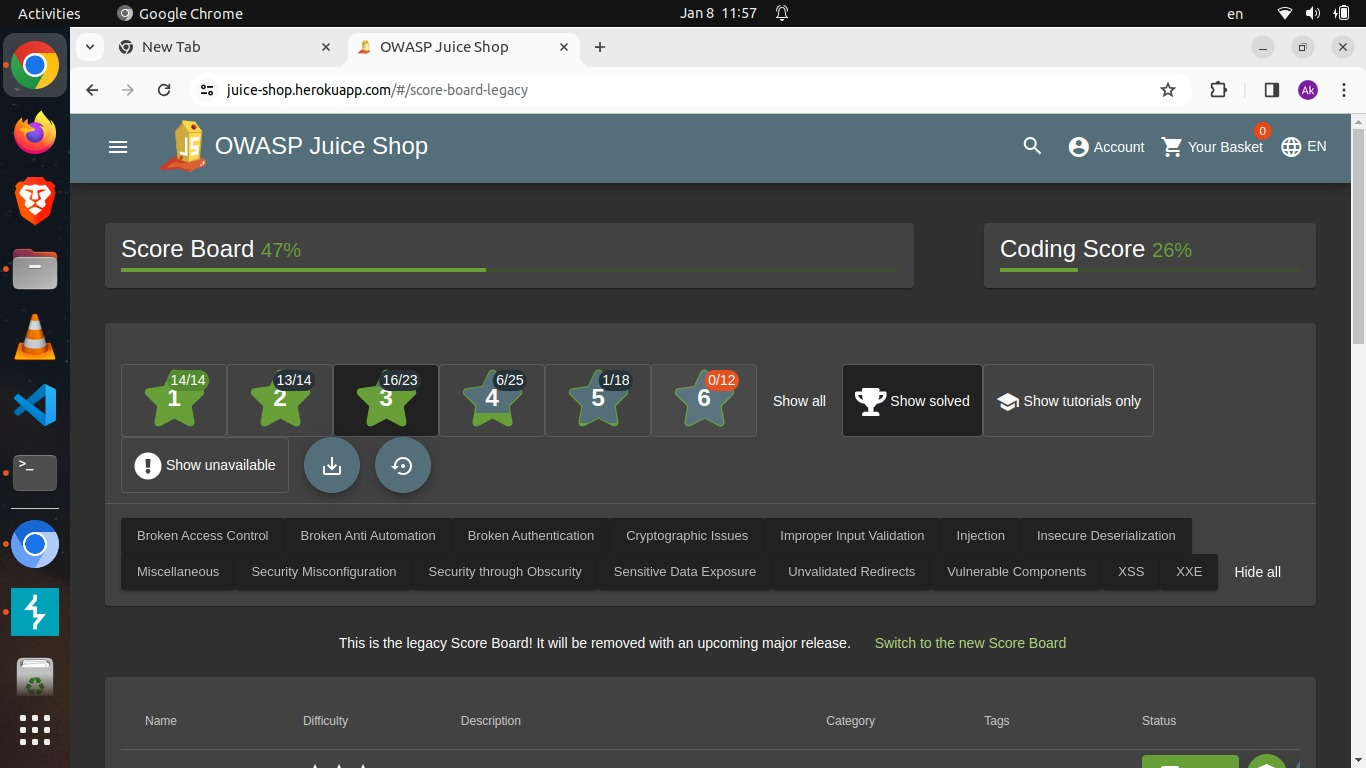
\includegraphics[width=1\linewidth]{images/image.png}
	\caption{сделаны работы на OWASP}
	\label{fig:mel-spec}
\end{figure}

\vspace{20pt}
{\let\clearpage\relax \chapter{Криптографические сбои}}

Первое, что нужно сделать, это определить потребности в защите данных при передаче и в состоянии покоя. Например, пароли, номера кредитных карт, медицинские записи, личная информация и коммерческая тайна требуют дополнительной защиты. Главным образом, если эти данные подпадают под действие законов о конфиденциальности, например, Общего регламента ЕС по защите данных (GDPR), или правил, например, защиты финансовых данных, таких как Стандарт безопасности данных индустрии платежных карт (PCI DSS). 

\vspace{20pt}
{\let\clearpage\relax \chapter{SQL инъекции}}

это один из очень распространённых способов взлома сайтов и веб‑приложений, работающих с реляционными базами данных.

Этот способ основан на внедрении в выполняемый приложением запрос к базе данных произвольного SQL‑кода, переданного злоумышленником. SQL‑инъекции являются одной из разновидностей атак типа «инъекция кода».

SQL‑инъекции, в зависимости от типа уязвимости, может дать возможность атакующему выполнить произвольный запрос к базе данных. То есть атакующий сможет прочитать содержимое любых таблиц, удалить, изменить или добавить данные, а также есть вероятность получения возможности работы с локальными файлами и выполнения произвольных команд на атакуемом сервере.\\

Последствия SQL‑инъекций:

\begin{enumerate}
    \item Кража данных;
    \item Модификация данных;
    \item Удаление данных;
    \item Полный взлом системы.
\end{enumerate}


\vspace{20pt}
{\let\clearpage\relax \chapter{Небезопасный дизайн}}

Небезопасный дизайн в веб приложении относится к ситуациям, когда архитектурные или дизайнерские решения приводят к потенциальным уязвимостям, которые могут быть использованы злоумышленниками для проведения атак. Эти недостатки могут оставить приложение открытым для различных угроз, таких как несанкционированный доступ, утечки данных, атаки на безопасность и другие виды атак.

\begin{enumerate}
    \item Недостаточная обработка аутентификации и авторизации;
    \item Недостаточная защита сессий;
    \item Недостаточная защита от межсайтовой подделки запроса (CSRF);
    \item Недостаточная защита от кросс сайтового скриптинга (XSS).
\end{enumerate}


\vspace{20pt}
{\let\clearpage\relax \chapter{Уязвимые и устаревшие компоненты}}

Уязвимые и устаревшие компоненты в веб приложении представляют собой наиболее распространенную категорию угроз. Эти компоненты могут быть подвержены различным уязвимостям, которые могут быть использованы злоумышленниками для получения несанкционированного доступа, кражи данных или повреждения системы.

Для снижения рисков, связанных с использованием уязвимых и устаревших компонентов, необходимо регулярно проводить оценку безопасности веб приложения и своевременно обновлять компоненты до последних версий.

\vspace{20pt}
{\let\clearpage\relax \chapter{Неправильная конфигурация безопасности}}

Неправильная конфигурация безопасности может привести к снижению эффективности защитных механизмов веб приложения, что может сделать его уязвимым для атак.

Для снижения рисков, связанных с неправильной конфигурацией безопасности, необходимо использовать стандартные конфигурации безопасности, а также регулярно проводить аудит безопасности веб приложения.

Сбои идентификации и аутентификации в веб приложении

Сбои идентификации и аутентификации могут привести к несанкционированному доступу к веб приложению.

Для снижения рисков, связанных со сбоями идентификации и аутентификации, необходимо использовать надежные механизмы аутентификации, а также регулярно обновлять пароли пользователей.

\vspace{20pt}
{\let\clearpage\relax \chapter{Нарушения целостности программного обеспечения и данных}}

Нарушения целостности программного обеспечения и данных могут привести к краже данных или повреждению системы.

Для снижения рисков, связанных с нарушениями целостности программного обеспечения и данных, необходимо использовать надежные механизмы защиты от несанкционированного доступа, а также регулярно проводить резервное копирование данных.


\vspace{20pt}
{\let\clearpage\relax \chapter{Сбои ведения журнала безопасности и мониторинга}}

Сбои ведения журнала безопасности и мониторинга могут затруднить обнаружение и расследование инцидентов безопасности.

Для снижения рисков, связанных со сбоями ведения журнала безопасности и мониторинга, необходимо использовать надежные системы ведения журнала безопасности и мониторинга, а также регулярно проверять их работоспособность.


\vspace{20pt}
{\let\clearpage\relax \chapter{Подделка запроса на стороне сервера}}


Подделка запроса на стороне сервера (SSRF) — это уязвимость, которая позволяет злоумышленнику заставить веб приложение выполнить произвольный запрос к другому серверу.

Для снижения рисков, связанных с SSRF, необходимо использовать безопасные методы обработки запросов от пользователей, а также ограничивать доступ пользователей к ресурсам, которые не должны быть доступны извне.

\section*{Заключение}

Рекомендации по снижению рисков, связанных с уязвимостями веб приложений

Для снижения рисков, связанных с уязвимостями веб приложений, необходимо предпринять следующие меры:

\begin{itemize}
    \item Регулярно проводить оценку безопасности веб приложения. Оценка безопасности должна включать в себя анализ уязвимостей веб приложения, а также оценку эффективности защитных механизмов.
    \item Своевременно обновлять компоненты веб приложения. Обновления компонентов часто содержат исправления уязвимостей безопасности.
    \item Использовать стандартные конфигурации безопасности. Стандартные конфигурации безопасности обеспечивают базовый уровень защиты веб приложения.
    \item Регулярно проводить аудит безопасности веб приложения. Аудит безопасности позволяет выявить и устранить уязвимости, которые могут быть не обнаружены при оценке безопасности.
    \item Использовать надежные механизмы аутентификации. Надежные механизмы аутентификации позволяют предотвратить несанкционированный доступ к веб приложению.
    \item Регулярно обновлять пароли пользователей. Актуальные пароли помогают защитить веб приложение от атак, основанных на подборе паролей.
    \item Использовать надежные механизмы защиты от несанкционированного доступа. Надежные механизмы защиты от несанкционированного доступа помогают предотвратить кражу данных или повреждение системы.
    \item Регулярно проводить резервное копирование данных. Резервное копирование данных позволяет восстановить данные в случае их повреждения или кражи.
    \item Использовать надежные системы ведения журнала безопасности и мониторинга. Надежные системы ведения журнала безопасности и мониторинга помогают обнаружить и расследовать инциденты безопасности.
    \item Использовать безопасные методы обработки запросов от пользователей. Безопасные методы обработки запросов от пользователей помогают предотвратить SSRF и другие атаки, основанные на манипуляциях с запросами от пользователей.
\end{itemize}

Реализация этих рекомендаций поможет снизить риски, связанные с уязвимостями веб приложений, и обеспечить их безопасность.